\documentclass{beamer}
\usepackage[T2A]{fontenc}
\usepackage[utf8]{inputenc}
\usepackage[russian]{babel}
\usepackage{color}
\usepackage{hyperref}
\usepackage{listings}
\usepackage{color}
\usepackage{graphicx}
\usepackage{mathtools}
\usepackage{bm}
\usetheme{default}

\newcommand{\prevGender}{78,87\%}
\newcommand{\prevAge}{3,69}

\setbeamertemplate{footline}[frame number]

\title{Определение демографических характеристик пользователей
социальных сетей на основе анализа их музыкальных интересов}
\author{\textbf{Семёнов~A.~C.,} \\ 
    группа: M4238, \\
    научный руководитель: Фильченков~A.~A., к.ф.-м.н.}
\institute{Университет ИТМО}
\date{\today}

\subject{Научно-исследовательская работа}

\begin{document}

\begin{frame}
  \titlepage
\end{frame}

\begin{frame}{Интернет и его пользователи}
  \begin{itemize}
      \item {Огромное число пользователей}
          \begin{itemize}
              \item {Facebook~--- $968 \cdot 10^{6}$ уникальных посещений сайта в день}
              \item {Vkontakte~--- $75 \cdot 10^{6}$ уникальных посещений сайта в день}
              \item {Instagram~--- $400 \cdot 10^{6}$ уникальных посещений сайта в месяц}
          \end{itemize}
      \item {Информация о пользователях находится в открытом доступе}
          \begin{itemize}
              \item {Текст, который пишут пользователи}
              \item {Фотографии пользователей}
              \item {Интересы: фильмы, музыка, хобби}
              \item {Страна, город, геолокация}
              \item {Пол, возраст}
              \item {И т.д}
          \end{itemize}
  \end{itemize}
\end{frame}

\begin{frame}{Задача профилирования пользователей}
  \begin{itemize}
      \item {Информация о пользователях часто является неполной или отсутствует}
      \item {Задача: определить отсутствующие характеристики по имеющимся (по музыке)}
      \item {Характеристики пользователей являются ключевыми признаками в рекомендательных системах}
      \item {Существует множество подходов к определению характеристик пользователей}
          \begin{itemize}
              \item {Информация о музыке пользователей используется не часто}
              \item {Метод, использующий музыкальные предпочтения, может помочь улучшить существующие алгоритмы}
          \end{itemize}
  \end{itemize}
\end{frame}

\begin{frame}{Задача определения характеристик пользователей}
    \begin{figure}
        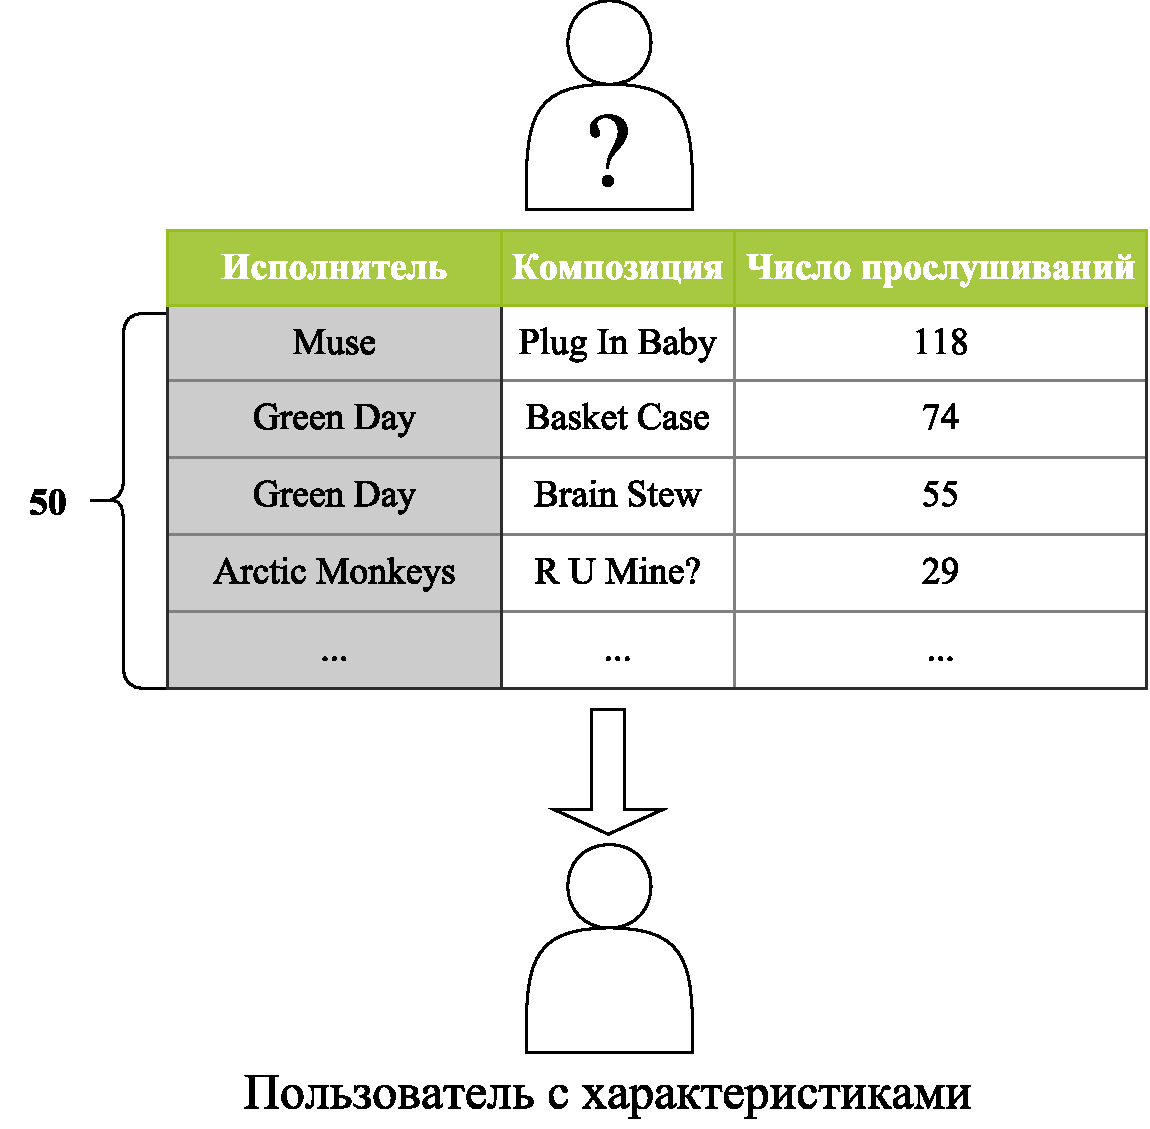
\includegraphics[scale=0.40]{figures/lastfm-top.pdf}
    \end{figure}
\end{frame}

\begin{frame}{Предлагаемый подход к решению}
    \begin{figure}
        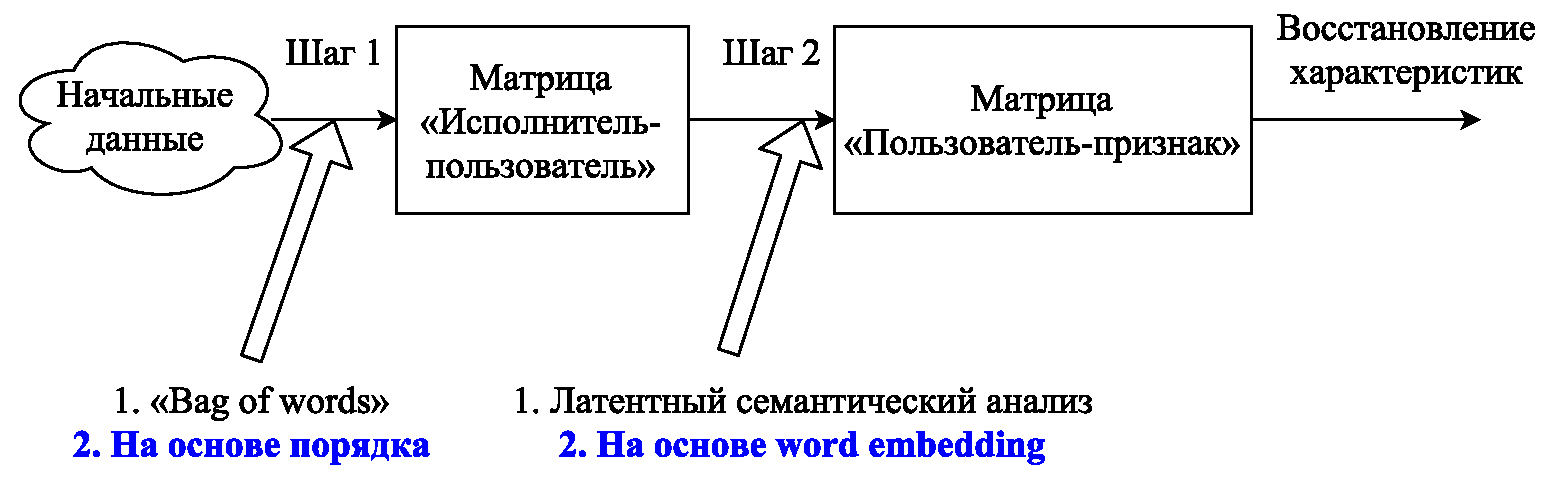
\includegraphics[width=\textwidth]{figures/master-concept.pdf}
    \end{figure}
\end{frame}

\begin{frame}{Шаг 1: <<bag of words>>}
  \begin{itemize}
      \item {Пользователи~--- документы, исполнители~--- термины}
      \item {$D = \{d_{ij}\}$~--- матрица термин--документ}
      \item {$d_{ij} = \mathrm{tf}_{ij} \cdot \log{\frac{n}{\mathrm{df}_{i}}}$ (Формула TF-IDF)}
          \begin{itemize}
              \item $\mathrm{tf}_{ij}$~--- число встреч термина $i$ в документе $j$
              \item $\mathrm{df}_{i}$~--- число документов, в которых встречается термин $i$
              \item $n$~--- общее число документов
          \end{itemize}
      \item {$d_{ij} = \begin{cases}
          0,& \mathrm{tf}_{ij} = 0,\\
          l(\mathrm{tf}_{ij}) \cdot g(\frac{n}{\mathrm{df}_{i}}),& \mathrm{tf}_{ij} \ne 0
      \end{cases}$}
          \begin{itemize}
              \item {$l(x), g(x)$~--- неубывающие неотрицательные функции}
          \end{itemize}
      \item {$ 
          d_{ij} = \log{(\mathrm{tf}_{ij} + 1)} 
          (1 + \sum_{j=1}^{n} \frac{p_{ij} \log{p_{ij}}}{\log{n}})
$ (Формула log-entropy)}
          \begin{itemize}
              \item {$p_{ij} = \frac{\mathrm{tf}_{ij}}{\mathrm{gf}_i}$}
              \item {$\mathrm{gf}_i$~--- общее число встреч термина $i$}
          \end{itemize}
  \end{itemize}
\end{frame}

\begin{frame}{Шаг 1: на основе порядка}
  \begin{itemize}
      \item {Гипотеза о значимости порядка следования исполнителей}
      \item {Чем выше находится исполнитель в списке,
               тем более <<значимым>> он является для пользователя}
      \item {Пусть $A_{ij} \subset \mathbb{N}$~--- множество позиций, на которых располагается
             исполнитель $i$ в списке у пользователя $j$}
      \item {$d_{ij} = \begin{cases}
          0,& A_{ij} = \varnothing,\\
          \sum\limits_{a \in A_{ij}}{f(a)},& A_{ij} \ne \varnothing 
      \end{cases}$}
      \begin{itemize}
          \item {$f(a)$~--- невозрастающая неотрицательная функция}
      \end{itemize}
  \end{itemize}
\end{frame}

\begin{frame}{Шаг 2: латентный семантический анализ}
  \begin{itemize}
      \item {Пусть $D \in \mathbb{R}^{m \times n}$~--- матрица исполнитель--пользователь}
      \item {\textit{Латентный семантический анализ}~--- пребразование документов из пространства
             терминов в пространство латентных тематик}
      \item {$D = U \cdot V^{T}$}
      \begin{itemize}
          \item {$U \in \mathbb{R}^{m \times k}$}
          \item {$V \in \mathbb{R}^{n \times k}$}
          \item {$k \ll m$}
          \item {$V$~--- матрица пользователь--признак}
      \end{itemize}
  \end{itemize}
\end{frame}

\begin{frame}{Шаг 2: на основе word embedding}
  \begin{itemize}
      \item {$D \in \mathbb{R}^{m \times n}$~--- исполнитель--пользователь}
      \item {\textit{Word embedding} преобразует термины в вектора произвольной размерности ($k$)}
      \item {$W \in \mathbb{R}^{m \times k}$~--- матрица, полученная при использовании word embedding}
      \item {$M = D^T \cdot W$}
      \begin{itemize}
          \item {$M \in \mathbb{R}^{n \times k}$}
          \item {$k \ll m$}
          \item {$M$~--- матрица пользователь--признак}
      \end{itemize}
  \end{itemize}
\end{frame}

\begin{frame}{Источник данных~--- Last.fm}
    \begin{figure}
        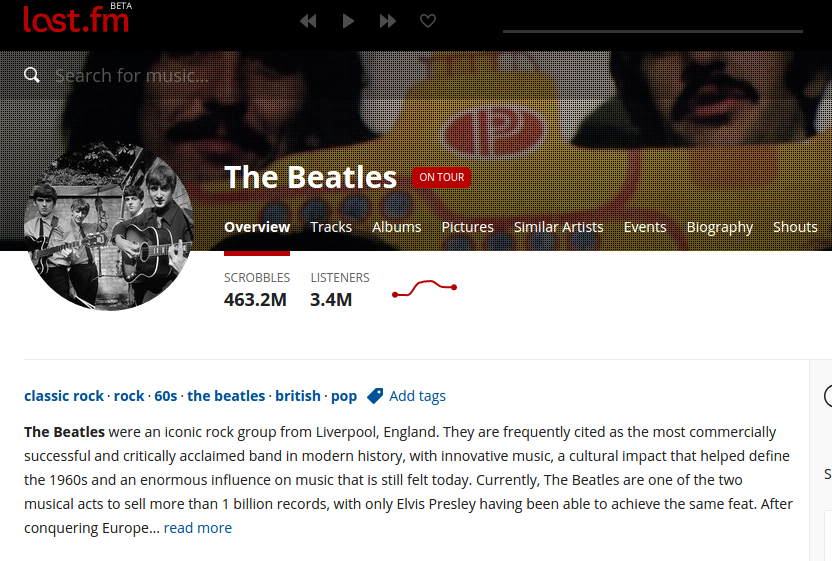
\includegraphics[width=\textwidth]{figures/lastfm.png}
    \end{figure}
\end{frame}

\begin{frame}{Подход на примере определения пола и возраста}
    \begin{itemize}
        \item {Использовался набор данных из существующего 
              исследования\footnote{Wu M. J.,
              Jang J. S. R., Lu C. H. Gender Identification
              and Age Estimation of Users Based on Music 
              Metadata // The International Society of Music Information Retrieval (ISMIR). – 2014. – P.~555--560.}}
        \item {Всего $96807$ пользователей}
            \begin{itemize}
                \item {48404 пользователей в обучающей выборке}
                \item {48403 пользователей в контрольной выборке}
            \end{itemize}
        \item {У каждого пользователя указан пол и возраст}
        \item {Пользователь описан исполнителями из top-50 наиболее
            прослушиваемых им композиций}
        \item {Особенности выборки}
            \begin{itemize}
                \item {66{,}2\% и 33{,}8\% мужчин и женщин соответственно}
                \item {Возраст пользователей смещён в сторону молодого поколения}
            \end{itemize}
    \end{itemize}
\end{frame}

\begin{frame}{Конфигурация используемых алгоритмов}
  \begin{itemize}
      \item {Определение пола~--- задача бинарной классификации}
          \begin{itemize}
              \item {Качество~--- точность}
          \end{itemize}
      \item {Определение возраста~--- задача восстановления регрессии}
          \begin{itemize}
              \item {Качество~--- средняя абсолютная ошибка}
          \end{itemize}
      \item {Латентный семантический анализ~--- \textit{LSI} (200 признаков)}
      \item {Word embedding~--- \textit{Word2Vec} (200 признаков)}
      \item {Метод опорных векторов с ядром \textit{RBF}}
      \item {Параметры $C$ и $\gamma$ настраивались методом \textit{Grid Search Cross Validation} на обучающей выборке}
      \item {Векторы пользователей были нормализованы перед использованием метода опорных векторов}
  \end{itemize}
\end{frame}

\begin{frame}{Результаты: <<bag of words>> + ЛСА}
    \[d_{ij} = \begin{cases}
              0,& \mathrm{tf}_{ij} = 0,\\
              l(\mathrm{tf}_{ij}) \cdot g(\frac{n}{\mathrm{df}_{i}}),& \mathrm{tf}_{ij} \ne 0
        \end{cases}\]

\begin{table}[!h]
\centering
\begin{tabular}{|c|c|c|c|}\hline
    \boldmath$l(x)$ & \boldmath$g(x)$ & \textbf{Определение пола} & \textbf{Определение возраста} \\\hline
    $1$ & $1$ & \textbf{82,46\%} & \textbf{3,54} \\\hline
    $\log{x}$ & $1$ & 81,59\% & 3,64 \\\hline
    $\log{x}$ & $\log{x}$ & 81,67\% & 3,58 \\\hline
    $\log{x}$ & $\sqrt{x}$ & 80,08\% & 5,49 \\\hline
    $\sqrt{x}$ & $1$ & 72,80\% & 4,79 \\\hline
    $\sqrt{x}$ & $\log{x}$ & 70,61\% & 4,91 \\\hline
    $\sqrt{x}$ & $\sqrt{x}$ & 67,07\% & 5,48 \\\hline
    $x$ & $1$ & 70,74\% & 5,02 \\\hline
    $x$ & $\log{x}$ & 69,38\% & 5,12 \\\hline
    $x$ & $\sqrt{x}$ & 67,44\% & 5,45 \\\hline
    \multicolumn{2}{|c|}{log-entropy} & 81,46\% & 3,59 \\\hline
\end{tabular}
\end{table}
\end{frame}

\begin{frame}{Результаты: матрица на основе порядка + ЛСА}
    \[d_{ij} = \begin{cases}
              0,& A_{ij} = \varnothing,\\
              \sum\limits_{a \in A_{ij}}{f(a)},& A_{ij} \ne \varnothing
          \end{cases}\]
\begin{table}[!h]
\centering
\begin{tabular}{|c|c|c|}\hline
    \boldmath$f(a)$ & \textbf{Определение пола} & \textbf{Определение возраста} \\\hline
    $\frac{1}{\log(a + 1)}$ & \textbf{79,65\%} & \textbf{3,93} \\\hline
    $\frac{1}{\sqrt{a}}$ & 79,39\% & 3,97 \\\hline
    $\frac{1}{a^2}$ & 77,51\% & 4,06 \\\hline
    $\frac{1}{a}$ & 77,67\% & 4,13 \\\hline
    $51 - a$ & 79,01\% & 3,98 \\\hline
    $\log{51} - \log{a}$ & 78,73\% & 4,04 \\\hline
    $\sqrt{51} - \sqrt{a}$ & 79,02\% & 4,01 \\\hline
\end{tabular}
\end{table}
\end{frame}

\begin{frame}{Результаты: <<bag of words>> + word embedding}
    \[d_{ij} = \begin{cases}
              0,& \mathrm{tf}_{ij} = 0,\\
              l(\mathrm{tf}_{ij}) \cdot g(\frac{n}{\mathrm{df}_{i}}),& \mathrm{tf}_{ij} \ne 0
        \end{cases}\]
\begin{table}[!h]
\centering
\begin{tabular}{|c|c|c|c|}\hline
    \boldmath$l(x)$ & \boldmath$g(x)$ & \textbf{Определение пола} & \textbf{Определение возраста} \\\hline
    $1$ & $1$ & 78,98\% & 3,24 \\\hline
    $\log{x}$ & $1$ & 78,26\% & 3,30 \\\hline
    $\log{x}$ & $\log{x}$ & 78,05\% & 3,42 \\\hline
    $\log{x}$ & $\sqrt{x}$ & 78.01\% & 3.43 \\\hline
    $\sqrt{x}$ & $1$ & 78,21\% & 3,38 \\\hline
    $\sqrt{x}$ & $\log{x}$ & 78,03\% & 3,43 \\\hline
    $\sqrt{x}$ & $\sqrt{x}$ & 78.01\% & 3.43 \\\hline
    $x$ & $1$ & 78,12\% & 3,41 \\\hline
    $x$ & $\log{x}$ & 78,01\% & 3,43 \\\hline
    $x$ & $\sqrt{x}$ & 78,00\% & 3,43 \\\hline
    \multicolumn{2}{|c|}{log-entropy} & \textbf{83,86\%} & \textbf{2,65} \\\hline
\end{tabular}
\end{table}
\end{frame}

\begin{frame}{Результаты: порядок исполнителей + word embedding}
    \[d_{ij} = \begin{cases}
              0,& A_{ij} = \varnothing,\\
              \sum\limits_{a \in A_{ij}}{f(a)},& A_{ij} \ne \varnothing
          \end{cases}\]
\begin{table}[!h]
\centering
\begin{tabular}{|c|c|c|}\hline
    \boldmath$f(a)$ & \textbf{Определение пола} & \textbf{Определение возраста} \\\hline
    $\frac{1}{\log(a + 1)}$ & 78,56\% & 3,15 \\\hline
    $\frac{1}{\sqrt{a}}$ & 80,32\% & \textbf{2,99} \\\hline
    $\frac{1}{a^2}$ & 74,77\% & 4,42 \\\hline
    $\frac{1}{a}$ & \textbf{80,89\%} & 3,35 \\\hline
    $51 - a$ & 77,82\% & 3,49 \\\hline
    $\log{51} - \log{a}$ & 78,18\% & 3,40 \\\hline
    $\sqrt{51} - \sqrt{a}$ & 78,11\% & 3,42 \\\hline
\end{tabular}
\end{table}
\end{frame}

\begin{frame}{Заключение}
    \textit{BOW+WE}~--- <<bag of words>> + word embedding \\
    \textit{BOW+ЛСА}~--- <<bag of words>> + ЛСА \\
    \textit{baseline}~--- Wu M. J.,
        Jang J. S. R., Lu C. H. Gender Identification
        and Age Estimation of Users Based on Music 
        Metadata // The International Society of Music Information Retrieval (ISMIR). – 2014. – P.~555--560.
    \begin{table}[h!]
    \centering
    \begin{tabular}{|c|c|c|c|}
    \hline
    \textbf{Тип задачи} & \textbf{BOW+WE} & \textbf{BOW+ЛСА} & \textbf{baseline} \tabularnewline
    \hline
    Определение пола & \textbf{83,86\%} & 82,46\% & \prevGender \tabularnewline
    \hline
    Определение возраста & \textbf{2,65} & 3,54 & \prevAge \tabularnewline
    \hline
    \end{tabular}
    \label{tab:total_results}
    \end{table}
\end{frame}

\begin{frame}
    \titlepage
\end{frame}

\end{document}
